\section{Topological Preliminaries}
This section aims to set the playing ground of the thesis. Since Morse theory needs the topological spaces to be rather restricted and the goal is to relate Morse Homology to toplogical K-Theory, there is an urge to just not worry about topological nuances. However, for proofing things we still need the vocabulary of topological notions. This chapter serves to provide the notions and theorems with references whilst omitting the technical proofs. Steenrod itselfs writes in his article "A convenient category of topological spaces" \cite{Steenrod1967}:

\begin{quote}
"Our need is to be able to make a variety of constructions and to know that the results have goof properties without the tedious spelling out at each step of lengthy hypotheses such as countably paracompactm normal, completely regular, first axiom of countability, metrizable, and so forth. It may be good research technique and an enjoyable exercise to analyse the precise circumstances for which an argument works; but id a developing theory is to be handy for research workers and attractive to students, then simplicity of the fundamentals must be the goal."
\end{quote}
Whilst Steenrod argues for the category of \textit{compactly generated Hausdorff spaces} the standart nowdays is the category of \textit{compactly generated weekly Hausdorff spaces}. The latter has direct limits, whilst Steenrods doesn't. But enough of the preamble. Lets start constructing that convinient categorie. I will assume that all topological constructions that are tought in the compulsory section of a university are known. 
\subsection{Compactly Generated Weekly Hausdorff Spaces}
\begin{figure}
    \centering
    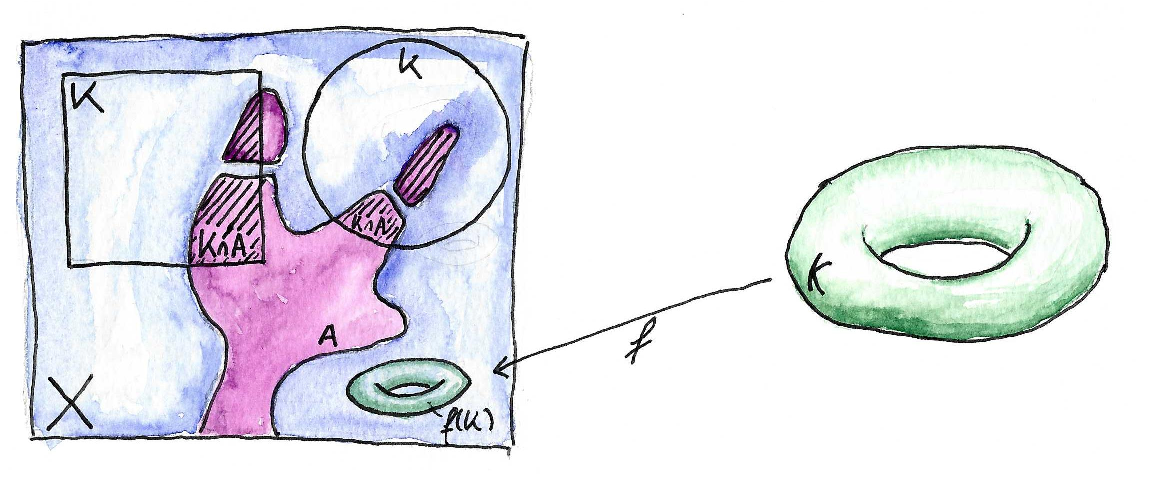
\includegraphics[width=\textwidth]{text/images/compactlyGeneratedWeakHausdorffTopology.pdf}
    The definition of compactly generated weak Hausdorff spaces.
\end{figure}
\begin{remark}[Notation and Convention]
    The literauter on topological spaces in geometric contextes is widly non unified. For this work, a topological space is \textit{compact} if it is quasi-compact (every open cover has a finite subcover) and Hausdorff (every pair of points can be seperated by disjoint open subsets). 
\end{remark}

\begin{definition}[Compactly Generated]\label{def:topPre-compactlyGenerated}
    A topological space $X$ is \textbf{compactly generated}, if a subset $A\subseteq X$ is closed, if and only if for all compact $K\subseteq X$ $A\cap K$ is closed. 
\end{definition}
\begin{definition}[Weak Hausdorff]\label{def:topPre-weakHausdorff}
    A topological space $X$ is called \text{weak Hausdoff}, if for all compakt Hausdorff spaces $K$ and continuous map $f:K\to X$ the image $\im(K)$ is compact in $X$. 
\end{definition}

\begin{definition}
    We call the category of compactly generated weak Hausforff spaces together with continuous functions as morphisms $\CGWH$. 
\end{definition}

\begin{proposition}
\begin{enumerate}
    \item Every closed subset of a compactly generated weak Hausdorff space is compactly generated weak Hausdorf in the subsettopology.
    \item Every locally compact Hausdorff space, and hence every compact space, is compactly generated weak Hausdorff.
    \item Every metric space is compactly generated.
    \item Every disjoint union of compactly generated weak Hausdorff spaces is compactly generated weak Hausdorff.
    \item If $X$ is compactly generated weak Hausdorff and $Y$ locally compact Hausdorff, then $X\times Y$ is compactly generated weak Hausforff in the product topology.
    \item If $X$ is compactly generated weak Hausdorff and $Y\subseteq X$ a closed subset of $X$. Then the quotionent topology on $X\big/ Y$ is compactly generated and weak Hausdorff.
\end{enumerate}
\begin{proof}
    For a proof we refer to Apendix A of \cite{schwede2018global}.
\end{proof}
\end{proposition}
There is another caveat and reason for the usage of $\CGWH$. If we view two CW-complexes as topological spaces, their product might not be a CW-complex. However as objects in $\CGWH$ their product is a CW-complex. The reason behind this is that the general product doesn't produce the final topology. That happens if the product topology is not compactly generated.(Such an example is found in \cite{BrookeTaylor2018}) If we enforce the latter by making the topology finer (which happens with categorical products in $\CGWH$) the product of CW-complexes is again a CW-complex. 
\begin{remark}
    From now on all topological spaces will be compactly generated weak Hausdorff.
\end{remark}

For the construction of toipological K-Theory we will heavily rely on the two theorems from pointset topology:
\begin{theorem}[Tietze Extension Theorem] Let $X$ be a normal space (and hence the theorem is true in $\CGWH$), $Y\subseteq X$ a closed subspace, $V$ a real vector space, and $f:Y\to V$ a continouos map. Then there exists a continuous map $g:X\to V$ such that $\restr{g}{Y}=f$.
\end{theorem}
\begin{theorem}[Existence of Partitions of Unity] Let $X$ be a compact space, $\{U_i\}$ a finite open covering. Then there exist continuous maps $f_i:X\to \R$ such that:
    \begin{enumerate}
        \item $f_i(x)\geq 0$ for all $x\in X$.
        \item $\supp(f_i)\subseteq U_i$.
        \item $\sum_i f_i(x)=1$ for all $x\in X$.
    \end{enumerate}
Such a collection $\{f_i\}$ is called a \textbf{partition of unity}.
\end{theorem}
\subsection{Topological Pairs}
\begin{figure}
	\centering
	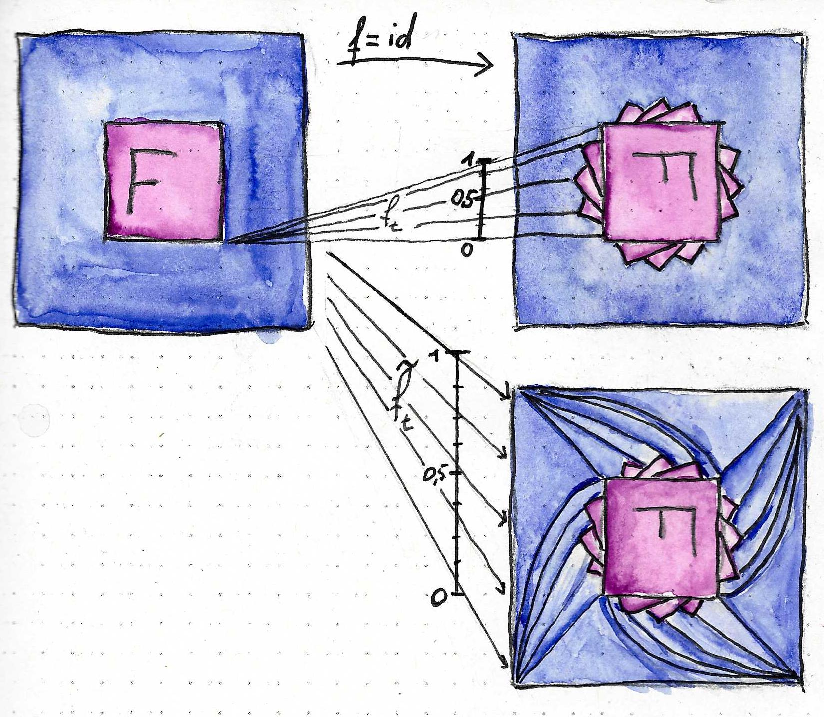
\includegraphics[width=0.7\textwidth]{text/images/homotopyExternsionProperty.pdf}
		\caption{ The homotopy extension property for the pair $(X,F)$, where $F$ gets rotated.}
\end{figure}
\begin{definition}[Homotopy Extension Property]
	Let $(X,A)$ be a topological pair, i,e, $A\subseteq X$. The pair satisfies the homotopy extension property if for any map $f:X\to Y$ and any homotopy $f_t:A\to Y$ with $f_0=\restr{f}{A}$ there exists an extension $\tilde{f}_t:X\to Y$ with $ \restr{\tilde{f}_t}{A}=f_t$ and $\tilde{f}_0=f$. The inclusiuon $i:A\to X$ of such a pair is called a \textbf{cofibration}.
\end{definition}
\begin{lemma}\label{lem:topPre-hepImpliescontractingisHomotopicalInvariant}
	If the pair $(X,A)$ satisfies the homotopy extension property and $A$ is contractible, then the quotient map 
	\begin{equation*}
		q: X\to X\big/ A
	\end{equation*} is an homotopy equivalence.
\end{lemma}
\begin{proof}
	Let $f_t:X\to X$ be a homtopy extending the conreaction of $A$ with $f_0=\id$. Then the composition $q\circ f_t$ maps $A$ to a point and hence factors over $X\big/A$ giving us the commutative diagram
	\begin{center}
		\begin{tikzcd}
			X \arrow[r,"f_t"] \arrow[d,"q"]& x \arrow[d,"q"]\\ 
			X\big/ A \arrow[r,"\overline{f_t}"']&X\big/ A
		\end{tikzcd}
	\end{center} Here, $\overline{f_t}$ dentoes the quotient map. Now $f_1(A)=pt$ where $pt$ is a point in $A$. So $f_1$ factors over $X\big/A$ and denote the induced map by $g:X\big/A \to X$. Now $g\circ q=f_1$ and hence 
	\begin{equation*}
		q\circ g(\overline{x})=q\circ g \circ q (x)=q\circ f_1 =\overline{f_1}(\overline{x})\,.
	\end{equation*} In other words we have the commutative diagram
	\begin{center}
		\begin{tikzcd}
			X \arrow[r,"f_1"] \arrow[d,"q"]& x \arrow[d,"q"]\\ 
			X\big/ A \arrow[r,"\overline{f_1}"']\arrow[ur,"g"] &X\big/ A
		\end{tikzcd}
	\end{center} This concludes the proof, since $g\circ q=f_1 \simeq f_0=\id$ and $q\circ g = \overline{f_1}\simeq \overline{f_0}=\id$.
\end{proof} 
\begin{definition}
    We call a pointed topological space $(X,x_0)$ well pointed, if the inclusion $x_0\to X$ is a cofibration. 
\end{definition}